\documentclass[journal]{IEEEtran}
\usepackage[a5paper, margin=10mm, onecolumn]{geometry}
\usepackage{lmodern} % Ensure lmodern is loaded for pdflatex
\usepackage{tfrupee} % Include tfrupee package

\setlength{\headheight}{1cm} % Set the height of the header box
\setlength{\headsep}{0mm}     % Set the distance between the header box and the top of the text

\usepackage{gvv-book}
\usepackage{gvv}
\usepackage{cite}
\usepackage{amsmath,amssymb,amsfonts,amsthm}
\usepackage{algorithmic}
\usepackage{graphicx}
\usepackage{textcomp}
\usepackage{xcolor}
\usepackage{txfonts}
\usepackage{listings}
\usepackage{enumitem}
\usepackage{mathtools}
\usepackage{gensymb}
\usepackage{comment}
\usepackage[breaklinks=true]{hyperref}
\usepackage{tkz-euclide} 
\usepackage{listings}                                      
\def\inputGnumericTable{}                                 
\usepackage[latin1]{inputenc}                                
\usepackage{color}                                            
\usepackage{array}                                            
\usepackage{longtable}
\usepackage{multicol}
\usepackage{calc}                                             
\usepackage{multirow}                                         
\usepackage{hhline}                                           
\usepackage{ifthen}                                           
\usepackage{lscape}
\begin{document}

\bibliographystyle{IEEEtran}
\vspace{3cm}

\title{9.1.5}
\author{EE24BTECH11004 - ANKIT JAINAR}
% \maketitle
% \newpage
% \bigskip
{\let\newpage\relax\maketitle}

\renewcommand{\thefigure}{\theenumi}
\renewcommand{\thetable}{\theenumi}
\setlength{\intextsep}{10pt} % Space between text and floats

\numberwithin{equation}{enumi}
\numberwithin{figure}{enumi}
\renewcommand{\thetable}{\theenumi}

\textbf{Question}:
Solve the differential equation$\frac{d^2y}{dx^2} = \cos(3x) + \sin(3x)$.
\newline
\textbf{Solution: }
\begin{table}[h!]    
  \centering
  \begin{tabular}{|l|l|l|}
\hline
\textbf{Component} & \textbf{Arduino Pin} & \textbf{Description} \\
\hline
\multicolumn{3}{|c|}{\textbf{LCD Display}} \\
\hline
RS & PB0 (Digital 8) & Register Select line \\
\hline
E & PB1 (Digital 9) & Enable line \\
\hline
D4 & PB2 (Digital 10) & Data line 4 \\
\hline
D5 & PB3 (Digital 11) & Data line 5 \\
\hline
D6 & PB4 (Digital 12) & Data line 6 \\
\hline
D7 & PB5 (Digital 13) & Data line 7 \\
\hline
\multicolumn{3}{|c|}{\textbf{7-Segment Display}} \\
\hline
Segment A & PD4 (Digital 4) & Segment A line \\
\hline
Segment B & PD5 (Digital 5) & Segment B line \\
\hline
Segment C & PD6 (Digital 6) & Segment C line \\
\hline
Segment D & PD7 (Digital 7) & Segment D line \\
\hline
Common HH\_1 & PC0 (Analog 0) & Hours tens digit common \\
\hline
Common HH\_2 & PC1 (Analog 1) & Hours ones digit common \\
\hline
Common MM\_1 & PC2 (Analog 2) & Minutes tens digit common \\
\hline
Common MM\_2 & PC3 (Analog 3) & Minutes ones digit common \\
\hline
Common SS\_1 & PC4 (Analog 4) & Seconds tens digit common \\
\hline
Common SS\_2 & PC5 (Analog 5) & Seconds ones digit common \\
\hline
\multicolumn{3}{|c|}{\textbf{Buttons}} \\
\hline
Toggle Button & PD2 (Digital 2) & For cycling through options \\
\hline
Select Button & PD3 (Digital 3) & For selecting options \\
\hline
\end{tabular}
  \label{tab1.1.2.2}
\end{table}
\newline
\textbf{Theoretical Solution:}
\begin{align}
    \frac{d^2y}{dx^2} &= \cos(3x) + \sin(3x) \\
    \frac{dy}{dx} &= \int \cos(3x)dx + \int \sin(3x)dx + c_1 \\
    &= \frac{\sin(3x)}{3} - \frac{\cos(3x)}{3} + c_1 \\
    y &= \int \left( \frac{\sin(3x)}{3} - \frac{\cos(3x)}{3} + c_1 \right) dx + c_2 \\
    &= -\frac{\cos(3x)}{9} - \frac{\sin(3x)}{9} + c_1x + c_2
\end{align}
\newline
Assuming the initial conditions $y\brak{0} = 0$ and $y^{\prime}\brak{0} = 0$\\
\newline
substituting the initial conditions:
\begin{align}
    y\brak{0} = 0 &\implies -\frac{\cos(0)}{9} - \frac{\sin(0)}{9} + c_1 \cdot 0 + c_2 = 0 \\
    c_2 &= \frac{1}{9} \\
    y^{\prime}\brak{0} = 0 &\implies \frac{\sin(0)}{3} - \frac{\cos(0)}{3} + c_1 = 0 \\
    c_1 &= \frac{1}{3}
\end{align}
Thus, the theoretical solution is:
\begin{align}
    y\brak{x} = -\frac{\cos(3x)}{9} - \frac{\sin(3x)}{9} + \frac{x}{3} + \frac{1}{9}
\end{align}
\newline

\textbf{Computational Solution:}
\newline
Consider the given linear differential equation:
\begin{align}
    \frac{d^2y}{dx^2} = \cos(3x) + \sin(3x)
\end{align}
Using discretization, the second-order derivative can be approximated as:
\begin{align}
    y^{\prime\prime}\brak{t+h} = y^{\prime\prime}\brak{t} + h \cdot \left( \cos(3t) + \sin(3t) \right)
\end{align}
\newline
To express this as a system of equations:
\begin{align}
    \vec{y}_{k+1} = \myvec{1 & h & \frac{h^2}{2}\\ 0 & 1 & h\\ 0 & 0 & 1} \cdot \vec{y}_k + \myvec{0\\ 0\\ h^2\left(\cos(3x_k) + \sin(3x_k)\right)}
\end{align}
\newline
By iterating over the time steps, the computational solution is computed. A comparison of theoretical and computational result is shown in the figure below.
\begin{figure}[h!]
   \centering
   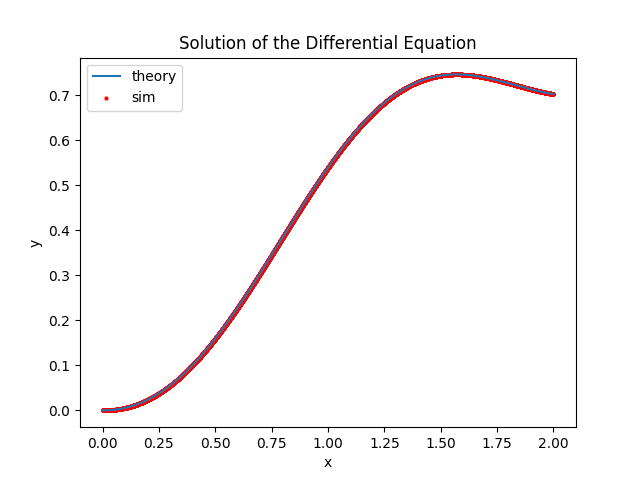
\includegraphics[width=\columnwidth]{figs/fig.png}
\end{figure}
\newline
\end{document}

